%&latex
%
\documentclass[../template.tex]{subfiles}
\begin{document}

\chapter{Limit Distributions}
In our previous discussion of Brownian motion, we concluded that the sum of many \textbf{independent}  \textit{gaussian} increments converges, in distribution, to a gaussian.

But what would happen if we consider increments that are still independent and identically distributed, but not gaussian? How would the distribution for their sum change, in the limit of \textit{many} steps? Does it even have a unique form?

\medskip

In this lesson, we will see that the sum of a general class of i.i.d. random variables - the ones for which it makes sense to compute mean and variance -, after some proper normalization, tends to a normal distribution. This is the gist of the \textbf{Central Limit Theorem} (CLT). 

Moreover, even the distributions without finite mean or variance, for which the CLT does not apply, can still produce sums that converge to some \textit{distribution} (not gaussian), which we call a \textbf{stable distribution}. This observation will allow us to study generalizations of Brownian motion, and in particular the phenomena of subdiffusion and superdiffusion, which have interesting physical applications.

\medskip

So, we will start by proving the CLT, and then generalize the diffusion equation and study it in some particular cases.

\section{Characteristic functions}
To prove the CLT, we first need a way to efficiently compute the pdf of a sum of i.i.d. random variables.

\medskip

Let's start with the case of just two \textbf{independent}  variables $X'$ and $X''$, with distributions $p_1(x')$ and $p_2(x'')$. Let $X = X' + X'' = f(X,X')$ be their sum, with distribution $p(x)$. 

Applying the rule for a change of random variables, we get:\marginpar{\vspace{1em}Sum of 2 independent random variables}
\begin{align} \label{eqn:sum-independent}
    p(x) &= \langle \delta(x-f(x',x'')) \rangle_{p_1,p_2} = \int_{\mathbb{R}} \dd{x'} \int_{\mathbb{R}} \dd{x''} p_1(x') p_2(x'') \delta(x-x'-x'')
\intertext{where we used the independence of $X'$ and $X''$ to factorize their joint pdf. By symmetry, $\delta(x-x'-x'') = \delta(x'+x''-x) = \delta(x''-(x-x'))$. Then, integrating over $x''$ to remove the $\delta$, we get:}
    &= \int_{\mathbb{R}} \dd{x'} \int_{\mathbb{R}} \dd{x''} p_1(x') p_2(x'') \delta(x''-(x-x')) = \int_{\mathbb{R}} \dd{x'} p_1(x') p_2(x-x') \nonumber
\end{align}
which is the \textbf{convolution} of the distributions $p_1$ and $p_2$.

\medskip

Convolutions are best computed in the Fourier domain, where they reduce to multiplications:
\begin{align} \label{eqn:conv-property}
    \mathcal{F}\left[\int_{\mathbb{R}} \dd{x'} p_1(x') p_2(x-x')\right](k) = \mathcal{F}[p_1](k) \cdot \mathcal{F}[p_2](k)
\end{align}
The Fourier transform\footnote{Here we are using a slightly different convention for the Fourier transform compared to sec. \ref{sec:fourier}, where both the $-$ sign and $(2\pi)^{-1}$ normalization factor are contained in the \textit{inverse} transform.} of a pdf $p(x)$ is called the \textbf{characteristic function}\index{Function!Characteristic} of the corresponding random variable $X$, and denoted with $\varphi(k)$:\marginpar{\vspace{1em}Characteristic function}
\begin{align*}
    \varphi(k) \equiv \mathcal{F}[p(x)](k) = \int_{\mathbb{R}} \dd{x} e^{ikx} p(x) = \langle e^{ikx} \rangle_{p(x)}
\end{align*} 
Note that $\varphi(k)$ is the \textit{moment-generating function} $M_X$ of $X$, evaluated at a complex argument:
\begin{align*}
    M_X(k) = \langle e^{kx} \rangle \Rightarrow \varphi(k) = M_X(ik)
\end{align*} 
This means that we can use $\varphi(k)$ to \textbf{compute moments}\marginpar{Moments from characteristic functions} of $X$. Note that:
\begin{align*}
    e^{ikx} = 1 + ikx -\frac{1}{2}k^2 x^2 + \dots = \sum_{n=0}^{+\infty} \frac{(ikx)^n}{n!}  
\end{align*}
And so:
\begin{align} \label{eqn:characteristic-expansion}
    \varphi(k) = \langle e^{ikx} \rangle = \sum_{n=0}^{\infty} \frac{i^n k^n}{n!} \langle x^n \rangle 
\end{align}
Then, by differentiating $n$ times and evaluating at $0$, all terms of order $\neq n$ vanish, leaving only a multiple of $\langle x^n \rangle$:
\begin{align*}
    \pdv{\varphi(k)}{k^n} &= \quad \mathclap{\underbrace{0}_{\text{{First n terms}}}} \quad + \> i^n \frac{n!}{n!} \langle x^n \rangle +\sum_{j=n+1}^{+\infty} \frac{n!}{j!} i^j k^{j-n} \langle x^j \rangle  =\\
    \pdv{\varphi(k)}{k^n} \Big|_{k=0} &= i^n \langle x^n \rangle \Rightarrow \langle x^n \rangle = \frac{1}{i^n} \textcolor{Red}{(-i^2)^n} \pdv{k^n}\varphi(k) \Big|_{k=0} = (-i)^n \pdv{k^n} \varphi(k) \Big|_{k=0} 
\end{align*}

\begin{expl}
    \textbf{Proof of convolution property}. Start from the left side of (\ref{eqn:conv-property}). By repeating backwards the steps from (\ref{eqn:sum-independent}) we have:
    \begin{align*}
        \mathcal{F}\left[\int_{\mathbb{R}} \dd{x'} p_1(x') p_2(x-x')\right](k) = \mathcal{F}\left[\int_{\mathbb{R}} \dd{x'} \int_{\mathbb{R}} \dd{x''} \delta (x-x'-x'')\right](k) = \span\\
        &= \int_{\mathbb{R}} \dd{x} e^{ikx} \int_{\mathbb{R}} \dd{x'}\int_{\mathbb{R}} \dd{x''} p_1(x') p_2(x'') \delta(x-x'-x'') =\\
        &= \int_{\mathbb{R}} \dd{x'} \int_{\mathbb{R}} \dd{x''} e^{ik(x'+x'')} p_1(x') p_2(x'') = \int_{\mathbb{R}} \dd{x'} e^{ikx'} \int_{\mathbb{R}} \dd{x''} e^{ikx''} = \\
        &= \mathcal{F}[p_1](k) \cdot \mathcal{F}[p_2](k)
    \end{align*}
\end{expl}

\section{Central Limit Theorem}
We are finally ready to prove the full Central Limit Theorem. 

\medskip

Consider a set of $n$ \textbf{independent} and \textbf{identically distributed} (i.i.d.) random variables $\bm{X} = \{X_1, \dots, X_n\}$, each according to a distribution $f(x)$ with \textbf{finite} mean $\mu$ and variance $\sigma^2$. We want to prove that their sum $S_n = \sum_{i=1}^n x_i$, when \textit{properly translated/scaled}, converges in distribution to a gaussian.

\medskip

More precisely, the \q{proper translation/scaling} means considering the random variable $Y_n$ defined by:
\begin{align}\label{eqn:yn-def}
    Y_n \equiv \frac{S_n - n \mu}{\sqrt{n} \sigma} 
\end{align} 

Note that, by additivity of mean and variance:
\begin{align*}
    \langle S_n \rangle &= \langle x_1 \rangle + \dots + \langle x_n \rangle = n \mu\\
    \operatorname{Var} (S_n) &= \operatorname{Var}(x_1) + \dots + \operatorname{Var}(x_n) = n \sigma^2 
\end{align*}
And so:
\begin{align*}
    \langle Y_n \rangle = \frac{\langle S_n \rangle - n \mu}{\sqrt{n} \sigma} = 0 \qquad \operatorname{Var}(Y_n) = \frac{\operatorname{Var}(S_n) }{n \sigma^2} = \frac{\cancel{n \sigma^2}}{\cancel{n \sigma^2}} = 1    
\end{align*}
where we used $\operatorname{Var}(x+a) = \operatorname{Var}(x)$ and $\operatorname{Var}(bx) = b^2 \operatorname{Var}(x)$ where $b \in \mathbb{R}$ is a constant. So, we expect $Y_n$ to converge in distribution to a standard gaussian ($0$ mean and unit variance).

\medskip

To compute the distribution of $Y_n$ we apply the rule for changing random variables:
\begin{align}\nonumber
    Y_n \sim g(y) &= \mathbb{P}(Y_n(\bm{x}) = y | x_i \sim f(x) \> \forall i) = \langle \delta(y- Y_n(x)) \rangle_{\bm{x} \sim [f(x)]^n} =\\
    \shortintertext{We rewrite the $\delta$ as a Fourier transform $\delta(x) = \mathcal{F}^{-1}[1] = (2 \pi)^{-1}\int_{\mathbb{R}} \dd{k} e^{-ikx}$, and then insert the definition for $Y_n$:} \nonumber
    &= \langle \frac{1}{2\pi} \int_{\mathbb{R}} \dd{\alpha} e^{-i \alpha(y - Y_n(\bm{x}))}  \rangle \underset{(\ref{eqn:yn-def})}{=} \langle \frac{1}{2\pi} \int_\mathbb{R} \dd{\alpha} \exp\left[-i \alpha y + i \alpha \left(\frac{\sum_{i=1}^n x_i - n \mu}{\sqrt{n} \sigma} \right)\right] \rangle =\\ \nonumber
    \shortintertext{By linearity we can bring the average inside the integral, which is then factorized as the $X_i$ are \textbf{independent}:} \nonumber
    &= \frac{1}{2\pi} \int_{\mathbb{R}} \dd{\alpha} \exp(-i \alpha y) \prod_{i=1}^n \langle \exp\left(\frac{i \alpha x_i}{\sqrt{n} \sigma} \right) \rangle \exp\left(-\frac{i \alpha n \mu}{\sqrt{n} \sigma} \right) =\\
    \shortintertext{Finally we write explicitly the average:} \nonumber
    &=  \frac{1}{2\pi} \int_{\mathbb{R}} \dd{\alpha} \exp\left(-i \alpha \left[y + \frac{n \mu}{\sqrt{n} \sigma} \right] \right) \prod_{i=1}^n \int_{\mathbb{R}} \dd{x_i} \exp\left(\frac{i \alpha x_i}{\sqrt{n} \sigma} \right) p(x_i) =\\ 
    \shortintertext{And then, as the $X_i$ are \textbf{identically} distributed, the product becomes the power of the characteristic function of \textit{any} of the $n$ variables:}
    &= \frac{1}{2\pi} \int_{\mathbb{R}} \dd{\alpha} \exp\left(-i \alpha \left[y + \frac{n \mu}{\sqrt{n} \sigma} \right]\right) \Bigg[\underbrace{\int_{\mathbb{R}} \dd{x_1} p(x_1) \exp\left(\frac{i \alpha x_1}{\sqrt{n} \sigma} \right)}_{\varphi_1\left(\frac{\alpha}{\sqrt{n} \sigma} \right)} \Bigg]^n \label{eqn:laststep}
\end{align}
As all the $n$ variables are effectively the same, we will drop the subscript in the following steps.

\medskip

The idea is now to expand $\varphi$ as in (\ref{eqn:characteristic-expansion}), bring all the terms inside the same exponential, and show that it reduces to a gaussian after integration. So:
\begin{align}\nonumber
    \varphi\left(k=\frac{\alpha}{\sqrt{n} \sigma} \right) &= 1 + i \underbrace{\langle x \rangle}_{\mu} \frac{\alpha}{\sqrt{n} \sigma} - \langle x^2 \rangle  \frac{\alpha^2}{2 n \sigma^2} + o(n^{-3/2})\\
    \shortintertext{This expansion only makes sense if $\mu$ and $\sigma$ are finite. Actually, we need to require  only $\sigma$  to be finite, as then $\mu$ is finite by consequence of the Cauchy Schwarz Inequality. To proceed, recall
that $\sigma^2 = \langle x^2 \rangle - \langle x \rangle^2 = \langle x^2 \rangle - \mu^2 \Rightarrow \langle x^2 \rangle = \sigma^2 + \mu^2$. Substituting in the previous expression:}
    &=\hlc{Yellow}{1 }+\hlc{SkyBlue}{ i \mu \frac{\alpha}{\sqrt{n} \sigma} - \frac{\alpha^2}{2n}} \hlc{ForestGreen}{- \frac{\alpha^2 \mu^2}{2 n \sigma^2}} + o(n^{-3/2}) = \label{eqn:midstep}\\
    \shortintertext{If we ignore all the higher order terms (as in the limit $n \to \infty$), (\ref{eqn:midstep}) is the expansion of the following exponential, as the only non-negligible terms are the three highlighted above:}
    &= \exp\left(\frac{i \alpha \mu}{\sqrt{n} \sigma} - \frac{\alpha^2}{2n} + o(n^{-3/2})  \right) \label{eqn:last2}
\end{align}
We then substitute (\ref{eqn:last2}) in (\ref{eqn:laststep}) and compute the $n$-th power:
\begin{align*}
    \mathbb{P}(Y_n(\bm{x}) = y) &= \frac{1}{2 \pi} \int_{\mathbb{R}} \dd{\alpha} \exp\left(-i \alpha \left[y + \frac{n \mu}{\sqrt{n} \sigma} \right]\right) \exp\left(\frac{i \alpha \mu n}{\sqrt{n} \sigma} - \frac{\alpha^2 n}{2 n} + o(n^{-1/2})  \right) =\\
    &= \frac{1}{2 \pi} \int_{\mathbb{R}} \dd{\alpha} \exp\left(-i \alpha y - \cancel{\frac{i \alpha n \mu}{\sqrt{n} \sigma}} + \cancel{\frac{i \alpha \mu n}{\sqrt{n} \sigma}} - \frac{\alpha^2}{2} + o(n^{-1/2})   \right) =\\
    &= \frac{1}{2\pi}\int_{\mathbb{R}} \dd{\alpha} \exp\left(-\frac{\alpha^2}{2} - i \alpha y + o(n^{-1/2}) \right) =
    \shortintertext{This is a gaussian integral, which evaluates, in the large $n$ limit, to:}
    &\underset{n \to \infty}{=}  \frac{1}{2\pi} \sqrt{\frac{\pi}{a} }  \exp\left(\frac{b^2}{4a} \right) = \frac{1}{\sqrt{2 \pi}} \exp\left(-\frac{y^2}{2} \right) 
\end{align*}
with $a = 1/2$ and $b = -iy$. The final result is the standard gaussian, as desired.

\medskip

So, we showed that if $X_i \sim p(x)$ with finite variance $\sigma$, then the sum of $n$ i.i.d. random variables $X_i$ converges in distribution to a gaussian:
\begin{align*}
    \lim_{n \to \infty} Y_n \sim \mathcal{N}(0,1)
\end{align*}
By undoing the normalization, we have:
\begin{align*}
    \lim_{n \to \infty} S_n \sim \mathcal{N}(n \mu, n \sigma^2)
\end{align*}
In particular, the sample mean distributes normally around the distribution mean $\mu$:
\begin{align*}
    \lim_{n \to \infty}\frac{1}{n} S_n  \mathcal{N}\left(\mu, \frac{\sigma^2}{n} \right)
\end{align*}

\section{Subdiffusion and superdiffusion}
Recall that, for Brownian motion, the final distribution for a particle starting in $x_0 = 0$ at $t_0 = 0$ is:
\begin{align*}
    W(x,t) = \frac{1}{\sqrt{4 \pi D t}}\exp\left(-\frac{x^2}{4 D t} \right)
\end{align*}
Its variance, which physically represents how quickly the initial distribution \q{spreads}, is linear in time:
\begin{align*}
    \langle x^2(t) \rangle = 2Dt
\end{align*}
This is indeed a good model for many physical phenomena. However, there are cases of \textbf{anomalous diffusion}, in which the \q{spreading velocity} scales \textit{differently} - as can be seen in fig. \ref{fig:levy}. For example:
\begin{itemize}
    \item \textbf{Subdiffusion}. Sometimes particles tend to persist in the same state for extended periods of time - meaning that the waiting time between \textit{jumps} has a distribution with a \q{long tail}, such as $t^{-1-\alpha}$ with $\alpha \in (0,1)$. This happens, for example, in the transport of charge carriers in semiconductors, and monomers in polymer diffusion. Their paths satisfy:
    \begin{align*}
        \langle x^2(t) \rangle = 2 D_{\zeta} t^{\zeta} \qquad 0 < \zeta < 1
    \end{align*}
    
    \item \textbf{Superdiffusion}. Here particles make jumps of large size with non-negligible frequency, meaning that the distribution of displacements $\Delta x$ has a \q{long tail}, proportional to $|\Delta x|^{-1 - \mu}$ for $\Delta x$ sufficiently large, with $\mu \in (0,2)$. If large jumps happen almost \textit{instantaneously}, we talk about \q{flights}, while if they happen with a fixed maximum velocity, they are \q{walks}. In this case we have:
    \begin{align*}
        \langle x^2(t) \rangle = 2 D_{\zeta} t^\zeta \qquad \zeta > 1
    \end{align*}
\end{itemize} 

\begin{figure}[!tbp]
    \begin{subfigure}[c]{0.45\textwidth}
      \centering
      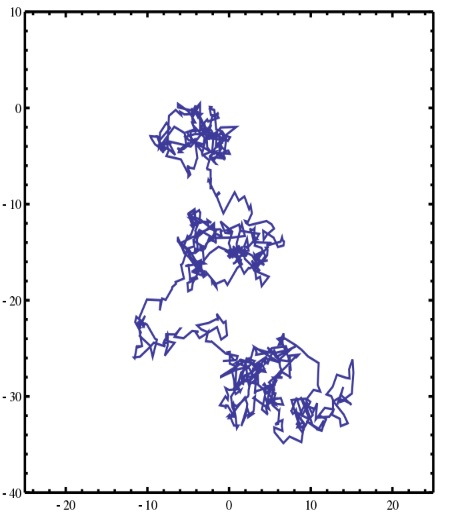
\includegraphics[width=0.8\textwidth]{Images/brownian.jpg}
      \caption{Brownian motion.}
      \label{fig:f1}
    \end{subfigure}
    \hfill
    \begin{subfigure}[c]{0.45\textwidth}
      \centering
      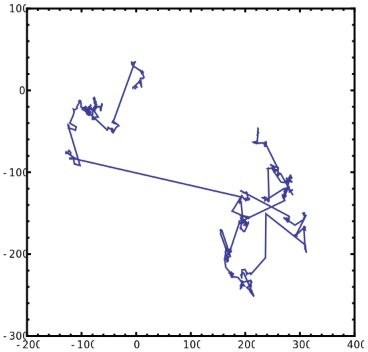
\includegraphics[width=0.9\textwidth]{Images/levy.jpg}
      \caption{Levy flight (superdiffusion). Note how jumps are frequently of very large size.}
      \label{fig:f2}
    \end{subfigure}
    \caption{Comparison between normal diffusion (a) and anomalous diffusion (b).\label{fig:levy}}
  \end{figure}
    
\section{Levy Flights}
Anomalous diffusion can be even more complicated, involving \textit{memory} and \textit{long-range correlations}. In our discussion, we will limit ourselves to
 a case of superdiffusion - the Levy flights - that can be described with a \textbf{generalized diffusion equation}:
\begin{align*}
    \begin{cases}
        \partial_t W(x,t) = D_{\mu} \pdv{|x|^\mu} W(x,t)\\
        W(x,0) = \rho(x)
    \end{cases} \qquad 0 < \mu < 2
\end{align*} 
The meaning of the \textit{fractional} derivative can be understood in Fourier space, as a generalization of the transform for a derivative:
\begin{align*}
    \partial_t \tilde{W}(k,t) ) = - D_{\mu} |k|^\mu \tilde{W}(k,t)
\end{align*}  
Note that this is equivalent to:
\begin{align*}
    \partial_t[\underbrace{e^{D_\mu |k|^\mu t} \tilde{W}(k,t)}_{\tilde{f}(k)} ] = D_\mu |k|^\mu\cancel{ e^{D_\mu |k|^\mu t}} \tilde{W}(k,t) + \cancel{e^{D_\mu |k|^\mu t}} \partial_t \tilde{W}(k,t) = 0
\end{align*}
Meaning that the function $\tilde{f}(k)$ is constant in time. Rearranging:
\begin{align*}
    \tilde{f}(k) \equiv \exp\left(D_\mu |k|^\mu t\right) \tilde{W}(k,t) \Rightarrow \tilde{W}(k,t) = \tilde{f}(k) e^{-D_\mu |k|^\mu t}
\end{align*}
As $\tilde{f}(k)$ does not depend on time, we can compute it at any instant, for example at $t=0$, where $\tilde{f}(k) = \tilde{W}(k,0) = \tilde{\rho}(k)$, and so:
\begin{align*}
    \tilde{W}(k,t) = \tilde{\rho}(k) \underbrace{e^{-D_\mu |k|^\mu t}}_{\tilde{W}(k,t|k_0,0)} 
\end{align*}
We interpret the exponential as the Fourier transform of a \textbf{propagator}. Multiplication in the Fourier domain corresponds to convolution in the space domain, and so we recover the usual form for the solution of the diffusion problem:
\begin{align*}
W(x,t) = \rho(x_0) * W(x,t|x_0,0)    
\end{align*}
And for $\mu = 2$ we know that:
\begin{align*}
    W(x,t) = \int_{\mathbb{R}} \dd{x_0} \rho(x_0) \underbrace{\frac{1}{4 D t} \exp\left(-\frac{(x-x_0)^2}{4Dt} \right)}_{W(x,t|x_0,0)} 
\end{align*}

For a general $\mu \in (0,2)$, however, it is difficult to find analytically $W(x,t|x_0,0)$, except for a few cases. One of them is for $\mu=1$, where $W(x,t)$ becomes a Cauchy distribution\marginpar{Cauchy Random Flights}, and we talk about \textbf{Cauchy random flights}:
\begin{align*}
    \tilde{W}_C(k,t) = \tilde{\rho}(k) e^{-D_1 |k| t} \Rightarrow W_C(x,t|0,0) &= \frac{1}{2\pi} \int_{\mathbb{R}} \dd{k} \exp\left(-x^*(t)|k| + ikx \right) =\\
    &= \frac{1}{\pi} \int_0^\infty \dd{k} e^{-x^*(t) k} \cos(kx) = \\
    &= \frac{1}{\pi x^*(t)} \frac{1}{\displaystyle 1+ \left(\frac{x}{x^*(t)} \right)^2}   
\end{align*} 
where we set $\rho(x) = \delta(x)$, and $x^*(t) = D_1 t$, representing the \textit{typical length scale}. See the exercises for a full derivation.

\medskip

Note that, in the case of Levy flights, the displacements \textit{do not follow} a distribution with finite variance, as it has a \q{long tail}. Thus, the CLT theorem does not apply, and in fact the sum of many displacements is not normally distributed - for example, in the $\mu=1$ case it is a Cauchy pdf.

\medskip

However, the Cauchy pdf has a key property in common with the gaussian: it is a \textbf{stable distribution}.\marginpar{Stable distributions} This means that a sum of two Cauchy random variables follows again a Cauchy pdf, up to scaling and translation.

\medskip

We argue (omitting the proof) that this property holds for all the distributions in the general case $\mu \in (0,2)$, which are called \textbf{Lévy alpha-stable distributions}. In particular, these stable distributions behave like \q{attractors}\marginpar{Generalized CLT theorem} for the sums of i.i.d. random variables with certain distributions, exactly like the gaussian behaves for all random variables with finite variance. This leads to a \textbf{generalization} of the central limit theorem, for which the sum of a number of random variables with symmetric distributions having power-law tails (Paretian tails), decreasing as $|x|^{-\alpha -1}$ for large $x$, with $\alpha \in (0,2]$ (and therefore with infinite variance), will tend to a Lévy stable distribution as the number of summands grows\footnote{B.V. Gnedenko, A.N. Kolmogorov. Limit distributions for sums of independent random variables, Cambridge, Addison-Wesley 1954 \url{https://books.google.com/books/about/Limit_distributions_for_sums_of_independ.html?id=rYsZAQAAIAAJ&redir_esc=y}\\ See Theorem 5 in Chapter 7, Section 35, page 181.}.


\end{document}
